% Options for packages loaded elsewhere
\PassOptionsToPackage{unicode}{hyperref}
\PassOptionsToPackage{hyphens}{url}
%
\documentclass[
]{book}
\usepackage{amsmath,amssymb}
\usepackage{lmodern}
\usepackage{iftex}
\ifPDFTeX
  \usepackage[T1]{fontenc}
  \usepackage[utf8]{inputenc}
  \usepackage{textcomp} % provide euro and other symbols
\else % if luatex or xetex
  \usepackage{unicode-math}
  \defaultfontfeatures{Scale=MatchLowercase}
  \defaultfontfeatures[\rmfamily]{Ligatures=TeX,Scale=1}
\fi
% Use upquote if available, for straight quotes in verbatim environments
\IfFileExists{upquote.sty}{\usepackage{upquote}}{}
\IfFileExists{microtype.sty}{% use microtype if available
  \usepackage[]{microtype}
  \UseMicrotypeSet[protrusion]{basicmath} % disable protrusion for tt fonts
}{}
\makeatletter
\@ifundefined{KOMAClassName}{% if non-KOMA class
  \IfFileExists{parskip.sty}{%
    \usepackage{parskip}
  }{% else
    \setlength{\parindent}{0pt}
    \setlength{\parskip}{6pt plus 2pt minus 1pt}}
}{% if KOMA class
  \KOMAoptions{parskip=half}}
\makeatother
\usepackage{xcolor}
\usepackage{longtable,booktabs,array}
\usepackage{calc} % for calculating minipage widths
% Correct order of tables after \paragraph or \subparagraph
\usepackage{etoolbox}
\makeatletter
\patchcmd\longtable{\par}{\if@noskipsec\mbox{}\fi\par}{}{}
\makeatother
% Allow footnotes in longtable head/foot
\IfFileExists{footnotehyper.sty}{\usepackage{footnotehyper}}{\usepackage{footnote}}
\makesavenoteenv{longtable}
\usepackage{graphicx}
\makeatletter
\def\maxwidth{\ifdim\Gin@nat@width>\linewidth\linewidth\else\Gin@nat@width\fi}
\def\maxheight{\ifdim\Gin@nat@height>\textheight\textheight\else\Gin@nat@height\fi}
\makeatother
% Scale images if necessary, so that they will not overflow the page
% margins by default, and it is still possible to overwrite the defaults
% using explicit options in \includegraphics[width, height, ...]{}
\setkeys{Gin}{width=\maxwidth,height=\maxheight,keepaspectratio}
% Set default figure placement to htbp
\makeatletter
\def\fps@figure{htbp}
\makeatother
\setlength{\emergencystretch}{3em} % prevent overfull lines
\providecommand{\tightlist}{%
  \setlength{\itemsep}{0pt}\setlength{\parskip}{0pt}}
\setcounter{secnumdepth}{5}
\usepackage{booktabs}
\ifLuaTeX
  \usepackage{selnolig}  % disable illegal ligatures
\fi
\usepackage[]{natbib}
\bibliographystyle{plainnat}
\IfFileExists{bookmark.sty}{\usepackage{bookmark}}{\usepackage{hyperref}}
\IfFileExists{xurl.sty}{\usepackage{xurl}}{} % add URL line breaks if available
\urlstyle{same} % disable monospaced font for URLs
\hypersetup{
  pdftitle={3 Pontos Sobre NBA},
  pdfauthor={Angelo Carmignani, Gabriel Bortoli, Wesley Maia},
  hidelinks,
  pdfcreator={LaTeX via pandoc}}

\title{3 Pontos Sobre NBA}
\author{Angelo Carmignani, Gabriel Bortoli, Wesley Maia}
\date{2023-07-13}

\begin{document}
\maketitle

{
\setcounter{tocdepth}{1}
\tableofcontents
}
\hypertarget{prefuxe1cio}{%
\chapter*{Prefácio}\label{prefuxe1cio}}
\addcontentsline{toc}{chapter}{Prefácio}

É com grande satisfação que apresento este trabalho de visualização de informação sobre dados da NBA, desenvolvido no âmbito da disciplina MAI5017 - Visualização de Informação, como parte integrante do Mestrado Profissional em Matemática, Estatística e Computação Aplicadas à Indústria (MECAI) do Instituto de Ciências Matemáticas e de Computação da Universidade de São Paulo.

A visualização de dados desempenha um papel crucial na análise e compreensão de conjuntos complexos de informações. No contexto do esporte, em particular, a visualização de dados tem se mostrado uma ferramenta poderosa para explorar e comunicar insights valiosos a partir de estatísticas e padrões relacionados aos jogos e aos jogadores de basquete.

Este trabalho tem como objetivo principal explorar os dados da NBA e utilizar técnicas de visualização para revelar informações significativas e interessantes sobre as partidas, os jogadores, as equipes e as tendências ao longo do tempo. Para tanto, foram utilizadas ferramentas e técnicas de programação em Python, um ambiente amplamente adotado no campo da ciência de dados e análise estatística.

A abordagem adotada neste trabalho segue o formato bookdown, uma estrutura que permite combinar narrativa, código e gráficos interativos de maneira integrada e coesa. Dessa forma, os resultados obtidos são apresentados de maneira clara e acessível, facilitando a compreensão e a exploração dos dados pelos leitores.

O estudo da visualização de informação aplicada à NBA não se restringe apenas ao interesse acadêmico, mas também possui um potencial significativo na indústria esportiva, na tomada de decisões estratégicas e no desenvolvimento de estratégias competitivas. Por meio da visualização eficaz de dados, é possível identificar padrões ocultos, analisar desempenhos individuais e coletivos, e extrair insights relevantes para apoiar a tomada de decisões informadas.

Agradeço a todos os professores e colegas do MECAI pelo apoio e incentivo ao longo desta jornada de aprendizado. Espero que este trabalho contribua para o avanço do conhecimento na área de visualização de informação e inspire pesquisas futuras no campo da análise de dados esportivos.

\hypertarget{author}{%
\chapter*{Sobre os Autores}\label{author}}
\addcontentsline{toc}{chapter}{Sobre os Autores}

\textbf{Gabriel Bortoli:} Formado em Ciência da Computação na UFSCar, atualmente trabalha na Kyndryl, em projetos internos de análise de dados e ciência de dados.

\textbf{Wesley Maia:} Formado em Bacharelado em Física na USP com MBA em Data Science \& Analytics pela USP, atualmente trabalha na Hand Talk como cientista de dados.

\hypertarget{introduuxe7uxe3o}{%
\chapter{Introdução}\label{introduuxe7uxe3o}}

A NBA (National Basketball Association) é uma das ligas de basquete mais populares e prestigiadas do mundo, com uma rica história que se estende por 77 anos. Desde sua fundação em 1946, a NBA tem sido palco de inúmeras façanhas atléticas, rivalidades intensas e momentos memoráveis que cativaram os fãs de basquete em todo o mundo.

Neste trabalho de Visualização de Dados, exploraremos um conjunto abrangente de estatísticas dos últimos 71 anos da NBA. Utilizando o Jupyter Notebook, mergulharemos nesses dados para extrair insights valiosos sobre as equipes, jogadores e padrões que moldaram a liga ao longo das décadas.

\hypertarget{objetivo}{%
\section{Objetivo}\label{objetivo}}

O objetivo desta análise é investigar diversas facetas do basquete profissional, desde o desempenho das equipes até as estatísticas individuais dos jogadores. Por meio de técnicas de análise de dados e visualização, buscaremos responder a perguntas como:

Quais equipes dominaram a NBA ao longo dos anos? Quais jogadores tiveram as melhores performances estatísticas em diferentes épocas? Existem tendências ou padrões significativos nas estatísticas da NBA ao longo das décadas? Como o jogo evoluiu em termos de estilo de jogo, pontuação média e estilos de arremesso? Ao responder a essas perguntas, esperamos obter uma compreensão mais profunda da evolução da NBA e das dinâmicas que impulsionam o sucesso das equipes e dos jogadores ao longo do tempo. Esses insights não apenas fornecerão informações interessantes sobre a história da liga, mas também poderão ajudar a prever tendências futuras e orientar estratégias para equipes e jogadores no presente.

\hypertarget{dados}{%
\chapter{Dados}\label{dados}}

O projeto tem um conjunto de dados fornecido pelo Kaggle chamado nba.csv. NA base apresenta os dados dos jogadores de todas as temporadas de 1951 a 2022, com um total de 33330 ocorrências

\hypertarget{descriuxe7uxe3o-da-base}{%
\section{Descrição da base}\label{descriuxe7uxe3o-da-base}}

As colunas são descritas a seguir:

POR JOGADOR:

\begin{longtable}[]{@{}
  >{\raggedright\arraybackslash}p{(\columnwidth - 2\tabcolsep) * \real{0.0935}}
  >{\raggedright\arraybackslash}p{(\columnwidth - 2\tabcolsep) * \real{0.9065}}@{}}
\toprule()
\begin{minipage}[b]{\linewidth}\raggedright
Variável
\end{minipage} & \begin{minipage}[b]{\linewidth}\raggedright
Descrição
\end{minipage} \\
\midrule()
\endhead
Rank & A classificação do jogador (ordenado por pontos marcados a cada temporada) \\
Year & O ano da temporada (por exemplo, ``2018-19'') \\
Season Start Year & O ano de início da temporada (por exemplo, 2018) \\
Season Type & Temporada regular ou playoffs \\
Player ID & Um ID gerado para cada jogador \\
Player & O nome do jogador \\
Team ID & ID gerado para cada equipe \\
Team & A equipe do jogador na respectiva temporada \\
Games Played & Jogos disputados na respectiva temporada \\
Minutes Played & Minutos jogados na respectiva temporada \\
FG Made & Cestas de campo convertidas (Field Goals Made) \\
FG Attempts & Tentativas de cestas de campo (Field Goals Attempted) \\
FG \% & Porcentagem de acertos de cestas de campo (Field Goal Percentage) \\
3-Pt FG Made & Cestas de três pontos convertidas (3 Point Field Goals Made) \\
3-Pt FG Attempts & Tentativas de cestas de três pontos (3 Point Field Goals Attempted) \\
3-Pt FG \% & Porcentagem de acertos de cestas de três pontos (3 Point Field Goal Percentage) \\
FT Made & Lances livres convertidos (Free Throws Made) \\
FT Attempts & Tentativas de lances livres (Free Throws Attempted) \\
FT \% & Porcentagem de acertos de lances livres (Free Throw Percentage) \\
Offensive Rebounds & Rebotes ofensivos \\
Defensive Rebounds & Rebotes defensivos \\
Rebounds & Total de rebotes (ofensivos + defensivos) \\
Assists & Assistências \\
Steals & Roubos de bola \\
Blocks & Tocos (bloqueios de arremessos) \\
Turnovers & Perdas de bola (erros) \\
Personal Fouls & Faltas pessoais \\
Points Scored & Pontos marcados \\
Efficiency & Eficiência calculada como (Pontos Marcados + Rebotes + Assistências + Roubos de Bola + Tocos - Chutes de Campo Perdidos - Lances Livres Perdidos - Perdas de Bola) dividido por Jogos Disputados \\
AST/TOV & Taxa de assistências para turnovers (Assist-to-Turnover ratio) \\
STL/TOV & Taxa de roubos de bola para turnovers (Steal-to-Turnover ratio) \\
\bottomrule()
\end{longtable}

\hypertarget{o-que-define-um-jogador-bom}{%
\chapter{O que define um jogador bom?}\label{o-que-define-um-jogador-bom}}

Para simplificação vamos utilizar o rank apresentado no dataset, que seriam os jogadores ordenados de acordo com a pontuação por temporada.

Apesar dessa rank não levar em consideração fatores defensivos, será feito uma avaliaçào se os maiores ``cestinhas'' também apresentam características defensivas acima da média.

A primeiro momento vamos avaliar como as informações estatísticas de cada jogador por temporada varia e como está relacionado com o rank. Para tanto será utiizado a técnica do PCA para entender melhor esse comportamento.

Para definir o número de componentes ideal foi availiada a variância explicada por cada componente e adotada a regra do cotovelo.

Pelo gráfico abaixo a partir da segunda componente já é explicada quase toda variância, sendo duas componentes suficiente para ter uma descrição dos dados, além de uma maior facilidade de interpretação visual dos dados.

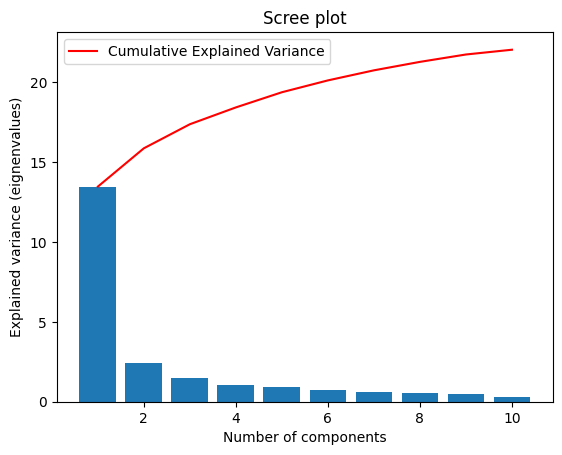
\includegraphics{imagens/3.png}

Na primeira análise do PCA é possível notar que as variáveis conseguem separar os jogadores mais bem ranqueados. Além disso, esse ranque pode seguir por três caminhos, todos com a variável eficiência sendo a principal, mas um mais voltado para cestas de dois, outros de três e por fim um voltado rebotes e bloqueios. Esse último principalmente para jogadores na função de pivôs e alas-pivôs.

Além disso, é possível notar que existem muitas variáveis correlacionadas, para futuras análises serão retiradas as que tiverem maior correlação e menor peso no PCA.

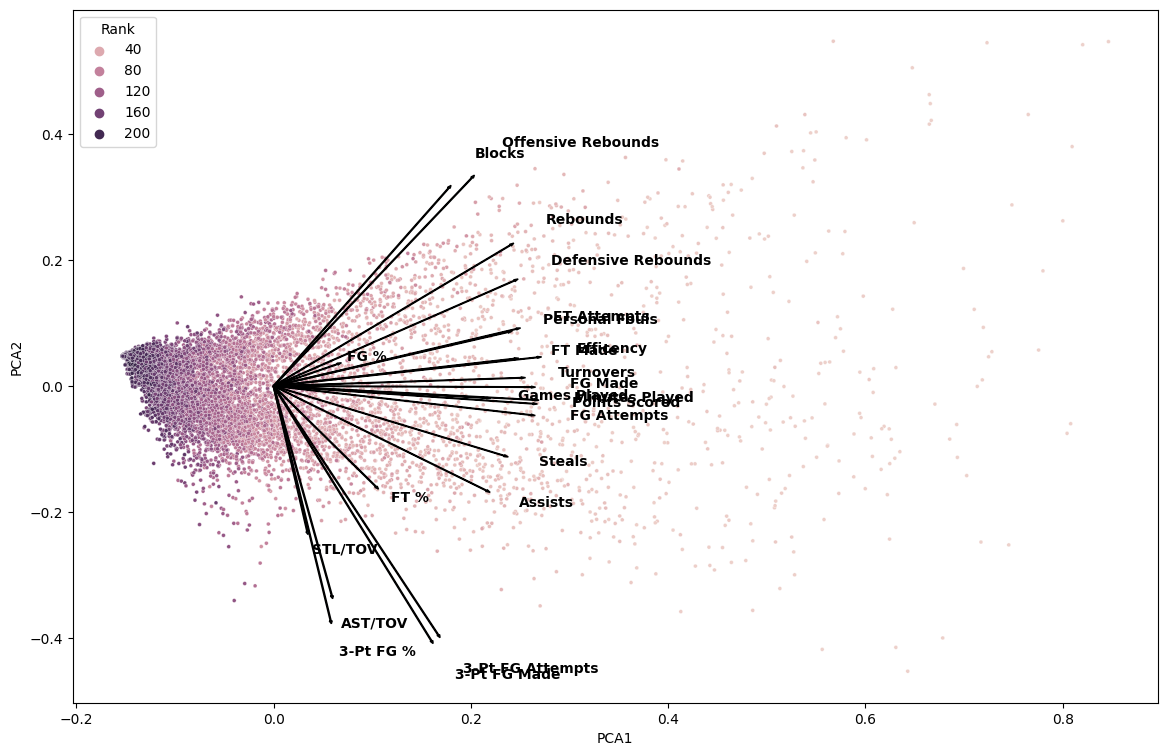
\includegraphics{imagens/4.png}

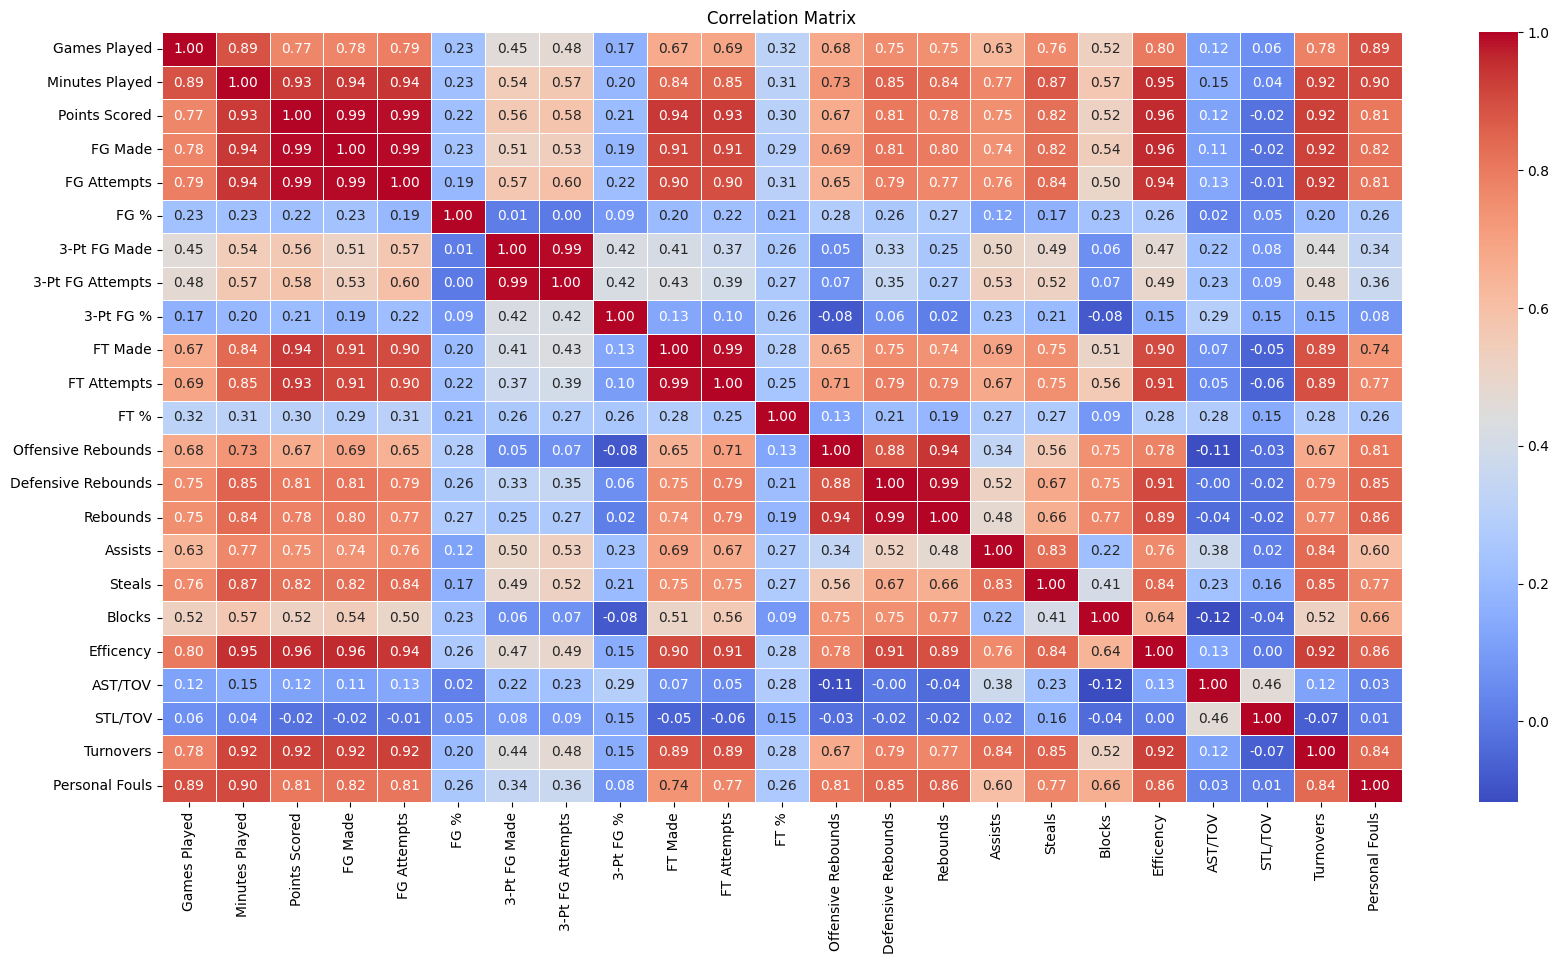
\includegraphics{imagens/5.png}

A matriz de correlação gerada mostra os coeficientes de correlação entre diferentes variáveis. Os valores na matriz variam de -1 a 1 e indicam a força e direção do relacionamento entre as variáveis.

Aqui estão algumas observações a partir da matriz de correlação:

Há uma forte correlação positiva entre ``Games Played'' e diversas outras variáveis como ``Minutes Played'', ``FG Made'', ``FG Attempts'', ``FT Made'' e ``FT Attempts''. Isso faz sentido, pois jogadores que jogam mais partidas tendem a acumular mais minutos e ter mais tentativas e sucessos em arremessos de quadra e lances livres.

Existe uma forte correlação positiva entre ``Offensive Rebounds'' e ``Defensive Rebounds'', o que é esperado, já que ambos contribuem para o número total de rebotes.

Há uma forte correlação positiva entre ``Points Scored'' e diversas outras variáveis como ``FG Made'', ``FT Made'' e ``Minutes Played''. Isso indica que jogadores que marcam mais pontos também tendem a converter mais arremessos de quadra, lances livres e atuam por mais minutos.

Após a redução de dimensionalidade é possível notar que ainda as estatísticas apresentam uma separação razoável na determinação do rank dos jogadores. Aliás, os maiores ranques são pontos bem distante do centroide. Na figura abaixo foi destacado os top 5 jogadores de cada temporada, além de trazer um exemplo para três jogadres: Lebron James, Shaquille O'Neal e Stephen Curry.

Interessante na avaliação dos três como o Curry se destaca pelas cestas dos três, O'Neal pela presença no garrafão, com elevado número de rebotes e o Lebron com uma das maiores eficiências já vistas na história da NBA.

Em resumo, para definição de um jogador bom é necessário uma maior eficiência como um todo, sendo que essa pode desviar de acordo com a posição e característica dos jogadores, seja sendo um armador com facilidade em cestas de 3 (Curry), um ala-pivô com característica mais equilibradas (Lebron) ou um pivô com uma presença no garrafão (O'Neal).

Por fim, mesmo o ranque utilizado ser de acordo com a pontuação, nota-se que os mais bem ranqueados nesse quesito não se destacam apenas por essa característica.

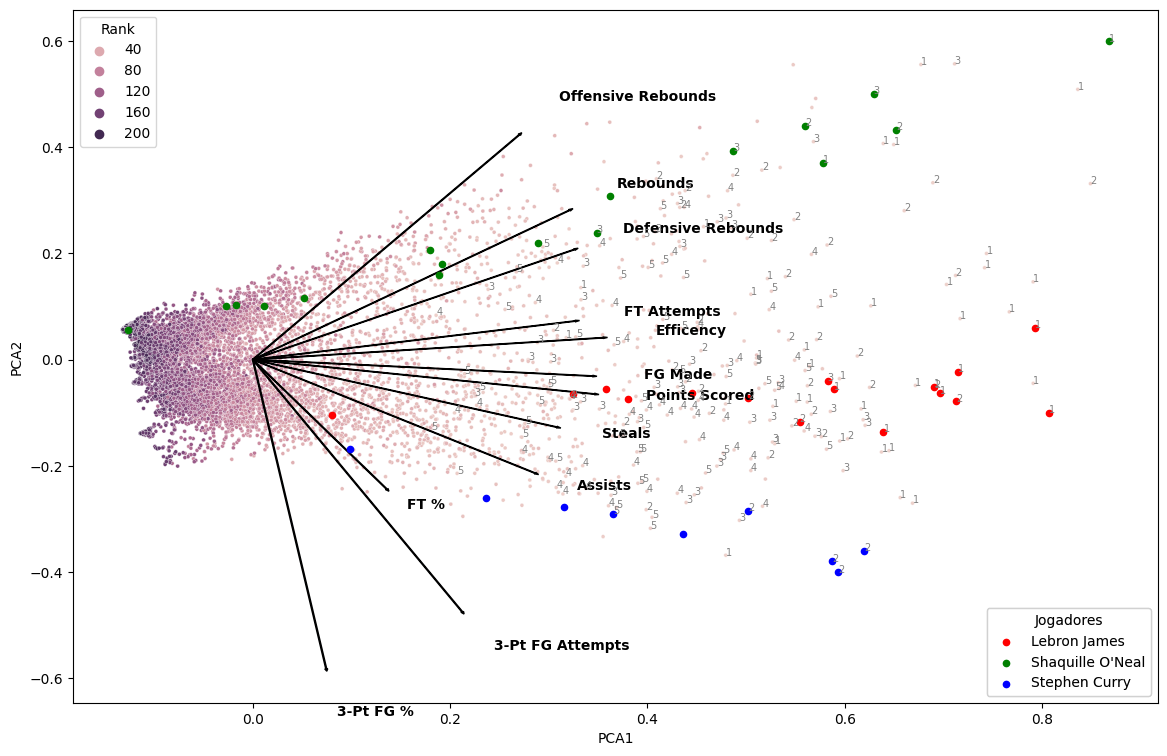
\includegraphics{imagens/6.png}

Para corroborar com a avaliação do PCA foi utilizada uma outra técnica a fim de verificar o poder de separação dos atributos da base, as Curvas de Andrews. Elas são úteis porque permitem identificar quais variáveis têm um maior impacto na separação dos grupos, ajudando a entender a importância relativa de cada característica. Além disso, elas também podem ser usadas para detectar a presença de outliers ou padrões incomuns nos dados.

As Curvas de Andrews são construídas utilizando a série de Fourier para transformar as variáveis originais em uma combinação de funções seno e cosseno. A série de Fourier é uma representação matemática de uma função periódica como uma soma infinita de funções seno e cosseno com diferentes frequências.

A fórmula da série de Fourier utilizada para construir as Curvas de Andrews é a seguinte:

Fórmula de Fourier para Curvas de Andrews

\(\ f(x) = \frac{a_0}{2} + \sum_{n=1}^{\infty} \left( a_n \cos(nx) + b_n \sin(nx) \right)\)

Nesta fórmula, f(x) representa a função que descreve a curva de Andre para uma determinada variável. Os coeficientes a\_0, a\_n e b\_n são calculados com base nos dados originais e representam a amplitude e a fase das funções seno e cosseno em diferentes frequências.

Para cada variável do conjunto de dados, a série de Fourier é aplicada e os coeficientes a\_0, a\_n e b\_n são determinados. Em seguida, as séries de Fourier são somadas para criar a curva de Andrews para cada grupo no conjunto de dados.

Essa abordagem permite representar as variáveis em termos de frequências harmônicas, revelando padrões e relações entre elas. As Curvas de Andrews resultantes são plotadas em um gráfico para visualização e análise da separação entre os grupos.

A interpretação das Curvas de Andrews é baseada na análise da forma das curvas e na distância entre elas. Se as curvas de diferentes grupos estão próximas umas das outras, isso indica que as variáveis têm um poder de separação menor. Por outro lado, se as curvas estão bem separadas, isso sugere que as variáveis têm um alto poder de separação entre os grupos.

Quando é observada a curva, é possível notar que as variáveis selecionaas no PCA apresentam uma boa separação entre os grupos top 20,top 21-70, 71-150 e maior que 150, indicando que esses atributos separam bem não somente os melhores jogadores, como destacados no PCA, mas também entre jogadores menos bem ranqueados.

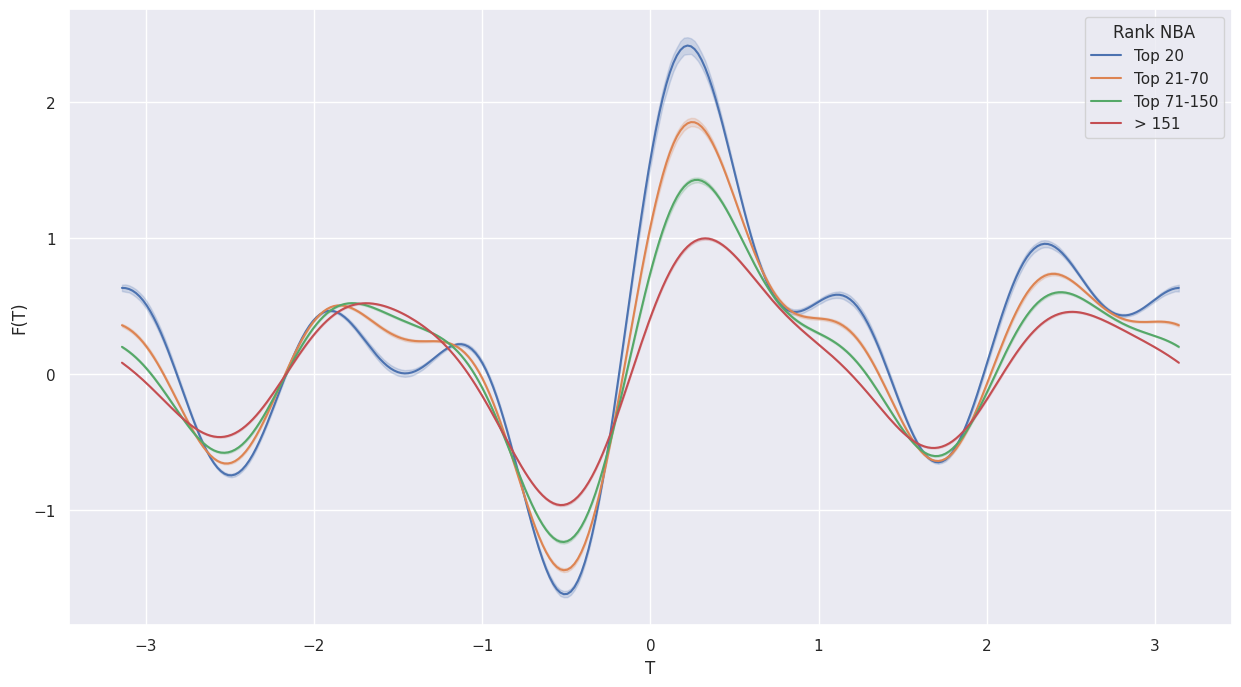
\includegraphics{imagens/7.png}

Por fim a última avaliação para os jogadores foi utilizando a técnica Radviz. Ele é um método de visualização utilizado para representar dados multivariados. Ele consiste em um gráfico circular no qual os pontos de dados são dispostos em torno de um círculo, sendo a posição de cada ponto determinada pelas suas variáveis. Cada variável é representada por um eixo radial, e a localização do ponto no gráfico indica a contribuição relativa de cada variável para o ponto de dados. Dessa forma, o Radviz permite identificar padrões e relacionamentos entre as variáveis de forma intuitiva e compacta.

Para o caso da NBA, uma propriedade interessante é quando um jogador se destaque em vários atributos, ele ficará mais ao centro do círculo, enquanto jogadores que se destacam mais por algum atributo específico tenderam a essa âncora.

Quando é observado os top 20 jogadores, é possível notar que estão mais concentrados ao centro, indicando que seus atributos não se limitam a uma habilidade específica, mas a apresentar um resultado razoável em todos os atributos. Além disso, conforme o ranque vai aumentando, os pontos vão ficando mais dispersos ao longo do círculo, indicando algum valor mais extremo.

Em resumo pelo Radviz, pode-se concluir que para ser bom na NBA não basta ser o cestinha, mas se destacar de maneira considerável em outros quesitos, como defesa, rebotes, variação de arremesos e assistências.

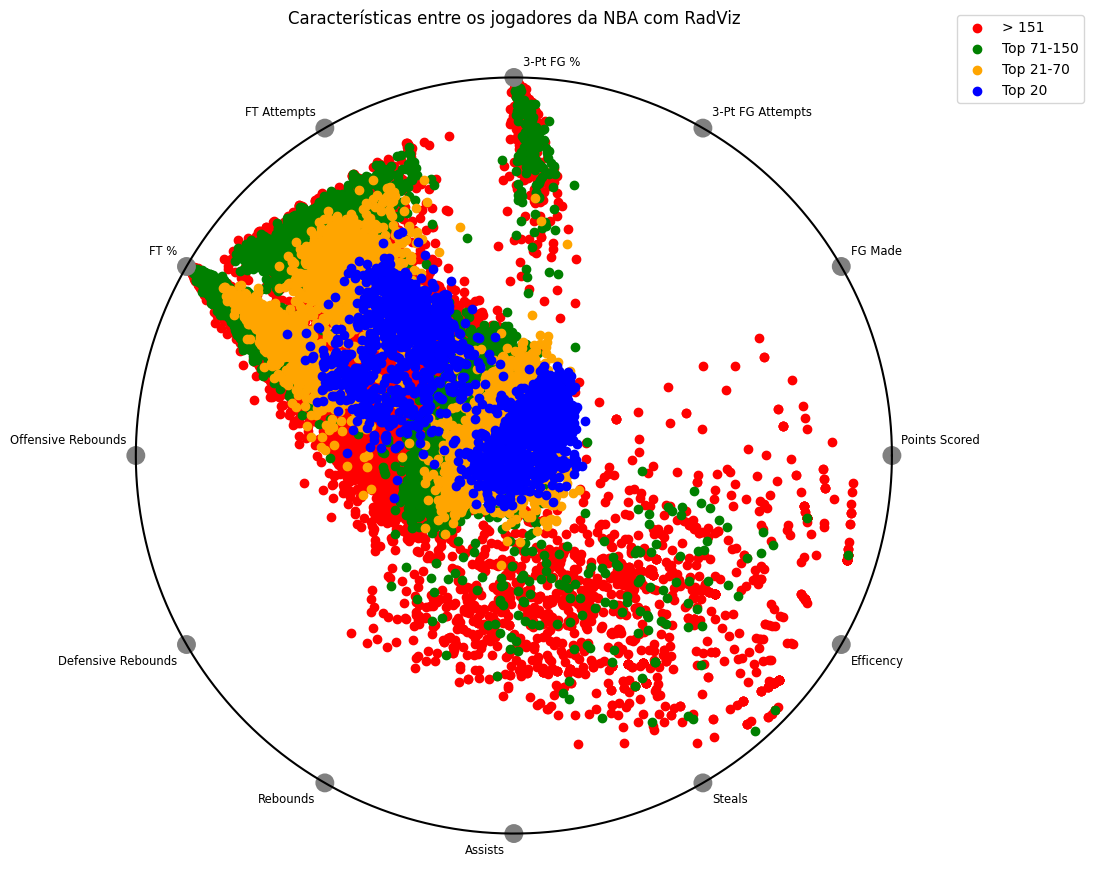
\includegraphics{imagens/download.png}

\hypertarget{evoluuxe7uxe3o-do-jogo-ao-longo-dos-tempos-e-temporadas.}{%
\chapter{Evolução do jogo ao longo dos tempos e temporadas.}\label{evoluuxe7uxe3o-do-jogo-ao-longo-dos-tempos-e-temporadas.}}

Ao avaliar o Radviz aberto por ano e temporada (regular e playoffs), é possível obter algumas conclusões:

\begin{itemize}
\tightlist
\item
  Na década de 80/90 os chutes de 3 eram menos frequentes. A variação desses dados é bem menor nesse período. É possível verificar essa análise ao avaliar as âncoras 3-pt FG\%, 3Pt FG Attempts e 3-pt FG Made, os quais não apresentam quase nenhum indicador tendendo a eles. Diferentemente das próximas décadas em que há uma dispersão bem maior tendendo a essas âncoras.
\item
  As informações são bem mais dispersas na temporada regular que nos playoffs, logo é mais difícil ter uma separação entre os jogares mais bem ranqueados, principalmente nos top 150.
\item
  Nos playoffs a dispersão dos dados é menor, sendo possível obter uma melhor separação para os top 20 jogadores. Importante notar que alguns extremos são jogadores até top 150, fato que não acontece na temporada regular.
\item
  Os top 20 jogadores da NBA, independente do ano ou da temporada sempre apresentam uma característica bem definida: são constante em todos indicadores, sem apresentar extremos.
\item
  Um exemplo disso é o Stephen Curry, muito conhecido pelos arremessos de 3 pontos, sempre bem ranqueado, porém se mantém próximo ao centro, uma vez que também é bem avaliado nos outros quesitos.
\end{itemize}

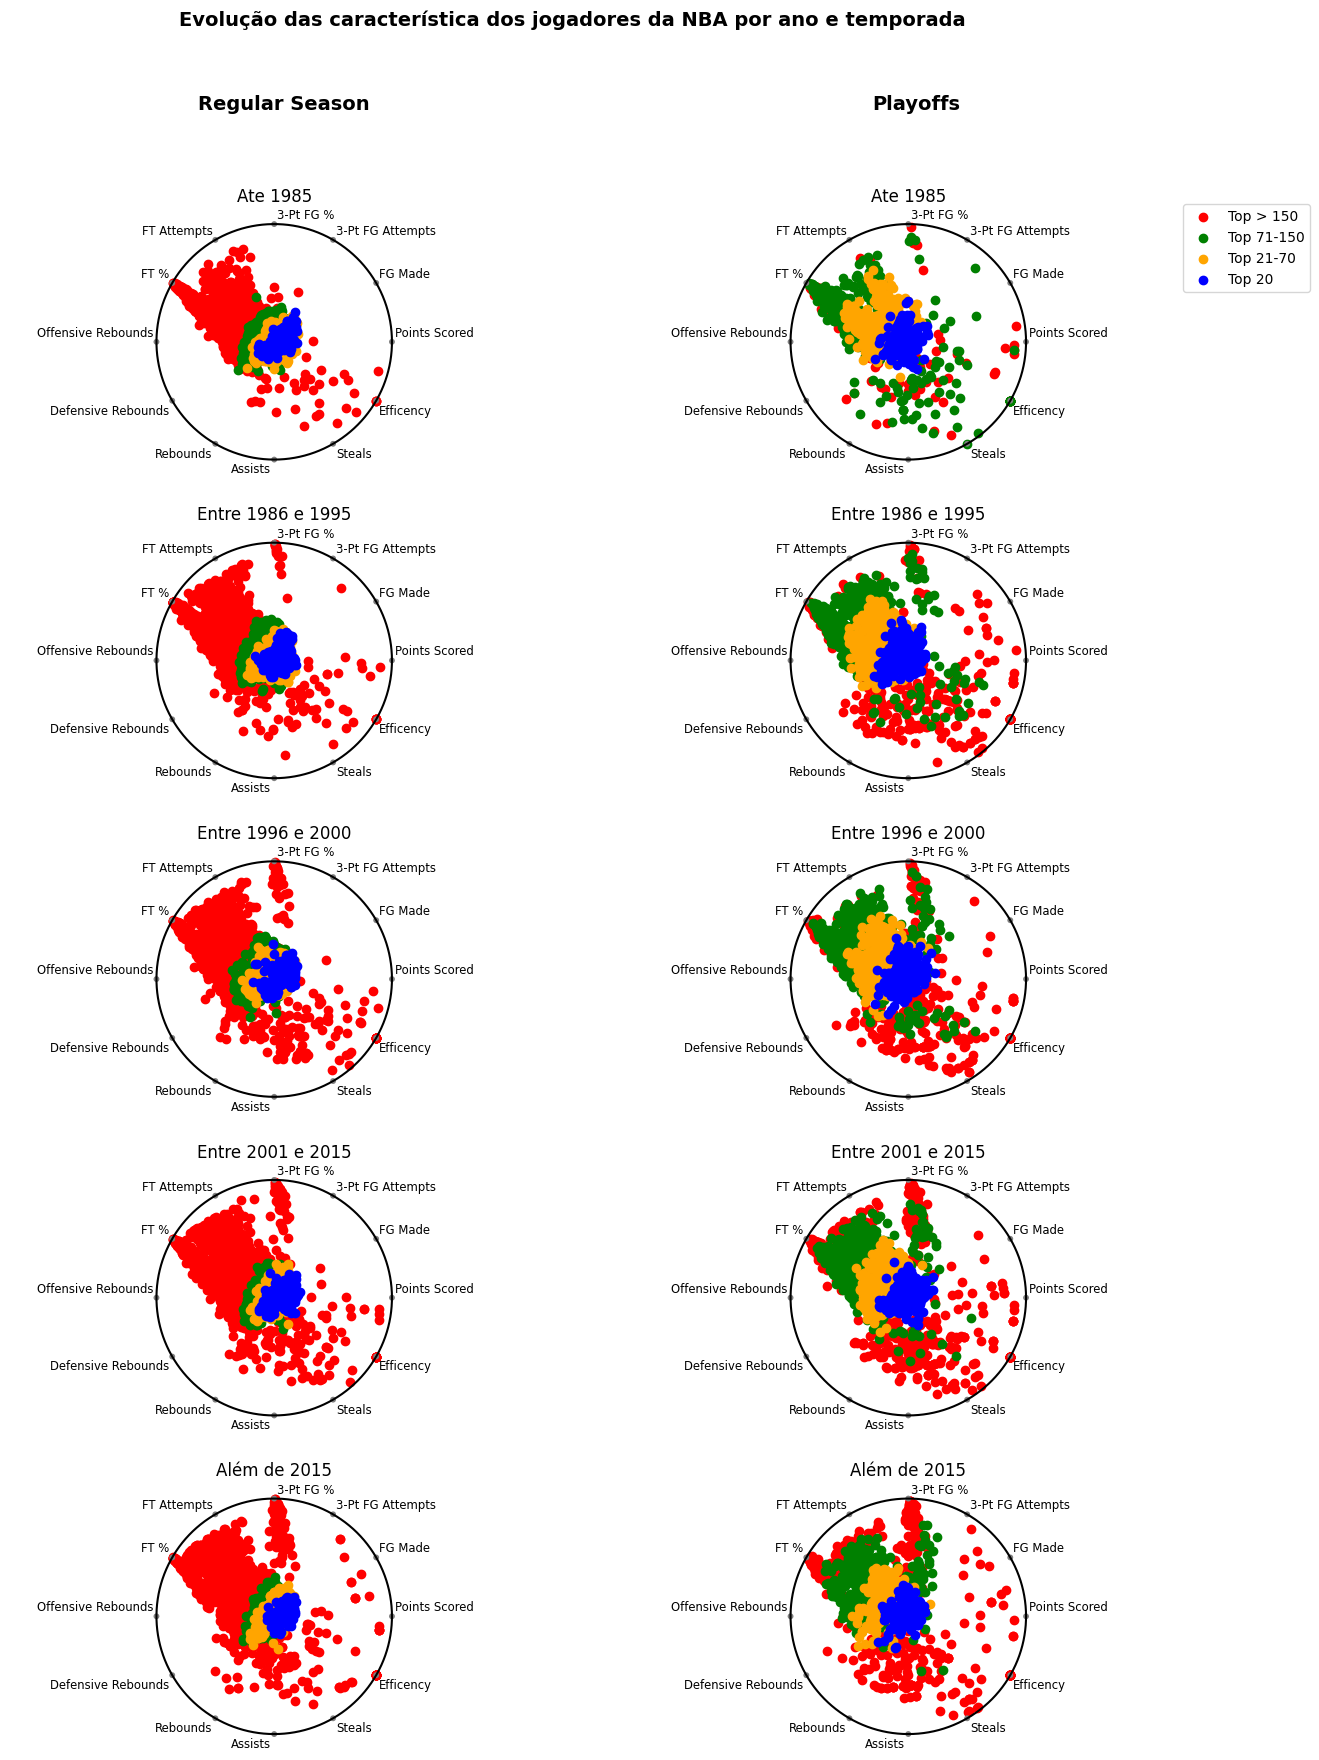
\includegraphics{imagens/14.png}

\hypertarget{principais-estatuxedstica-do-jogo}{%
\chapter{Principais estatística do jogo}\label{principais-estatuxedstica-do-jogo}}

Um maneira simples para entender melhor como um jogo de basquete funciona e como são os jogadores é avaliar as distribuições dos principais atributos. Quando os atributos são de características como, marcou mais pontos, arremesou mais, ou mais roubadas de bola, todos apresentam um formato exponencial, indicando que a tendência é que ao aumentar a frequência deles, uma menor quantidade de jogadores conseguem tal marca.

Além disso, é possível interpretar da forma que essa curva decai. Ao comparar arremessos de três frente a arremessos de dois pontos, a curva de três apresenta uma queda muito mais acentuada, indicando que é um atributo com menor frequência (ou de maior dificuldade). A mesma analogia pode ser aplicada para rebotes ofensivos e defensivos, sendo o primeiro muito menos frequente.

Por fim, os atributos de percentual de acerto de três pontos ou lances livres se assemelham a uma normal, indicando a característica do percentual de acerto de cada jogador. Importante destacar que a média de acertos em cestas de três é em torno de 35\%, enquanto de lances livres é de 80\%, evidenciando a maior dificuldade no acerto em cestas de três.

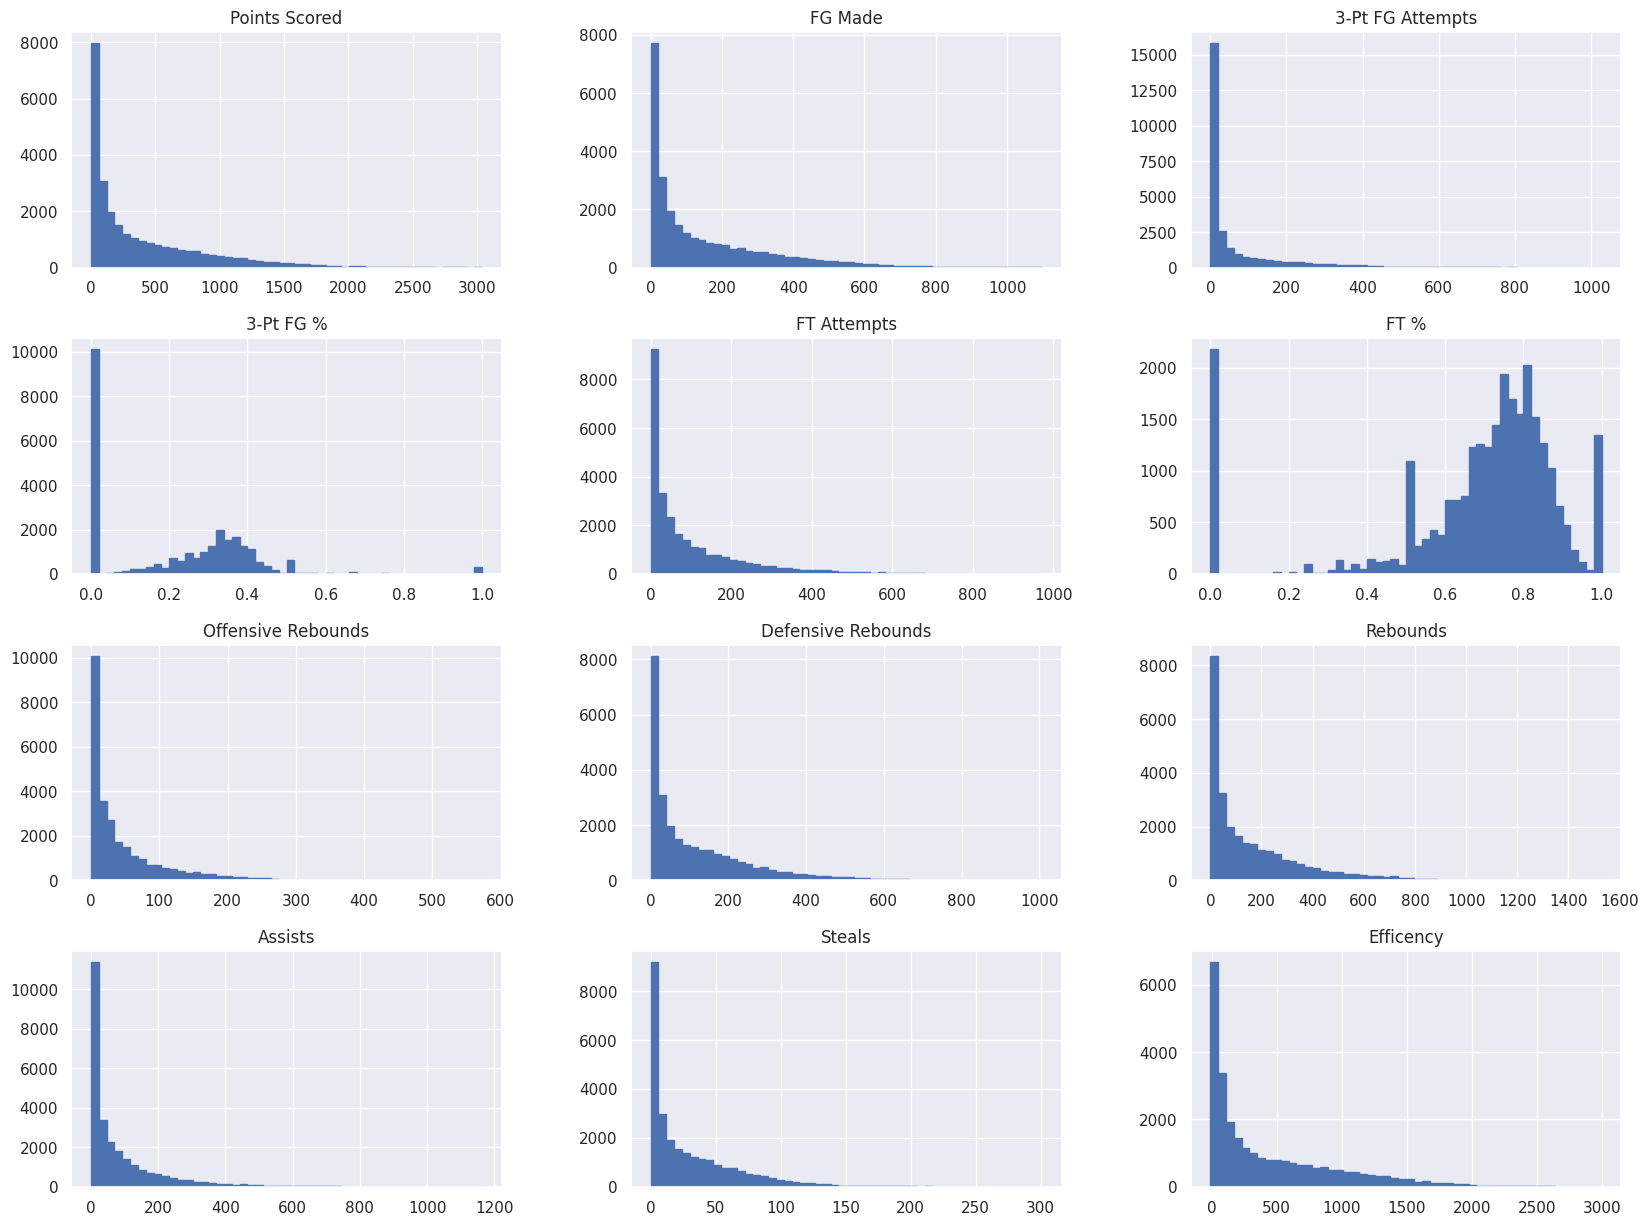
\includegraphics{imagens/15.png}

\textbf{Principais pontuadores de todos os tempos}

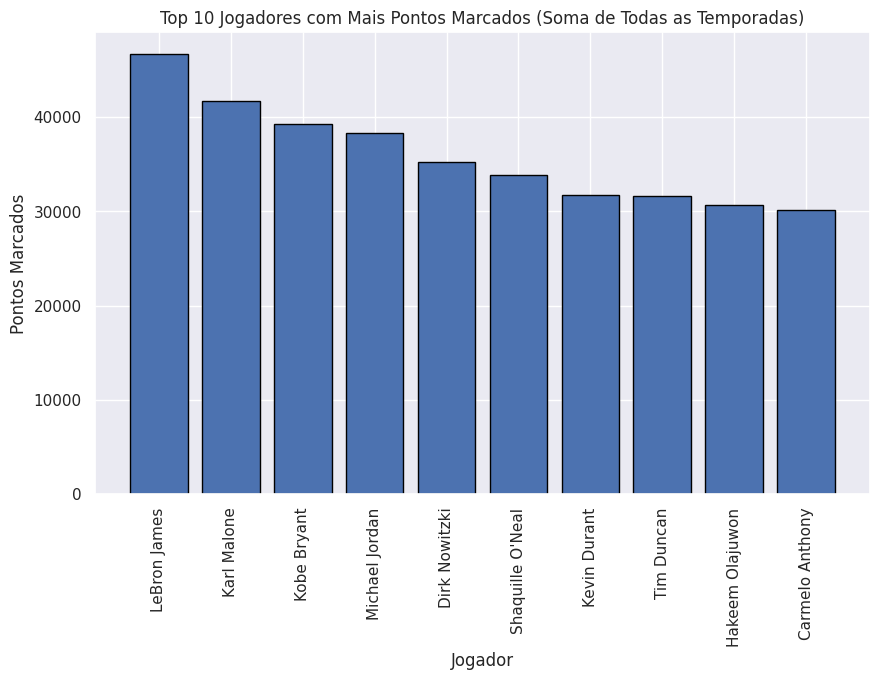
\includegraphics{imagens/16.png}

\textbf{Principais ``garçons'' de todos os tempos}

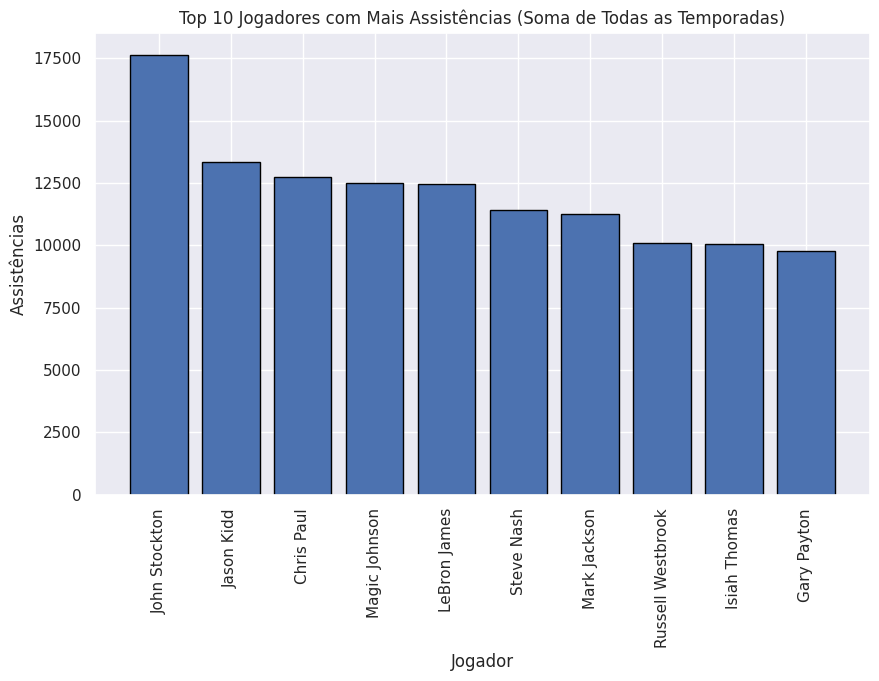
\includegraphics{imagens/17.png}

\textbf{Principais bloqueadores de todos os tempos}

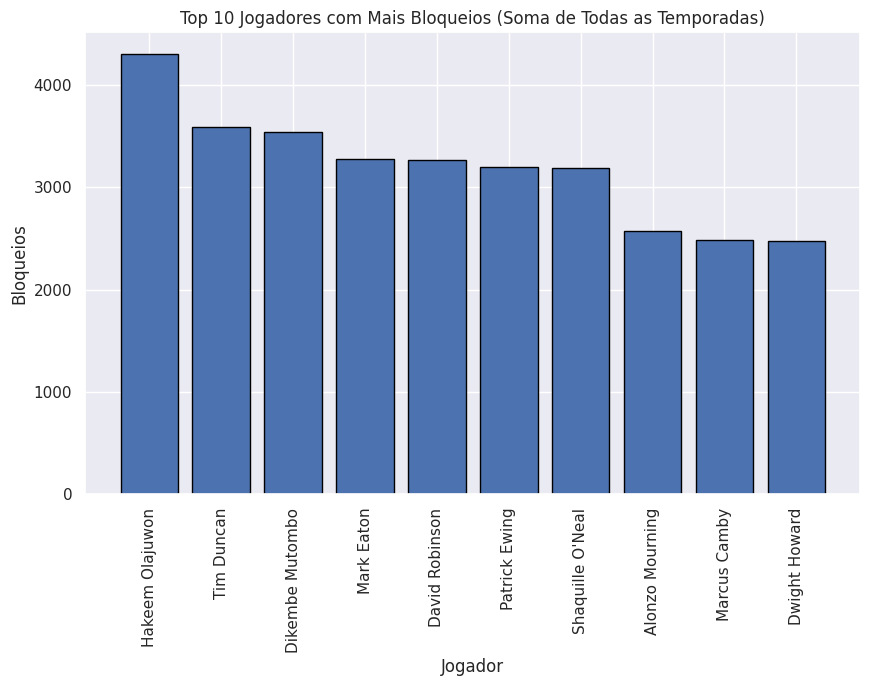
\includegraphics{imagens/18.png}

\textbf{Principais pontuadores dos três de todos os tempos}

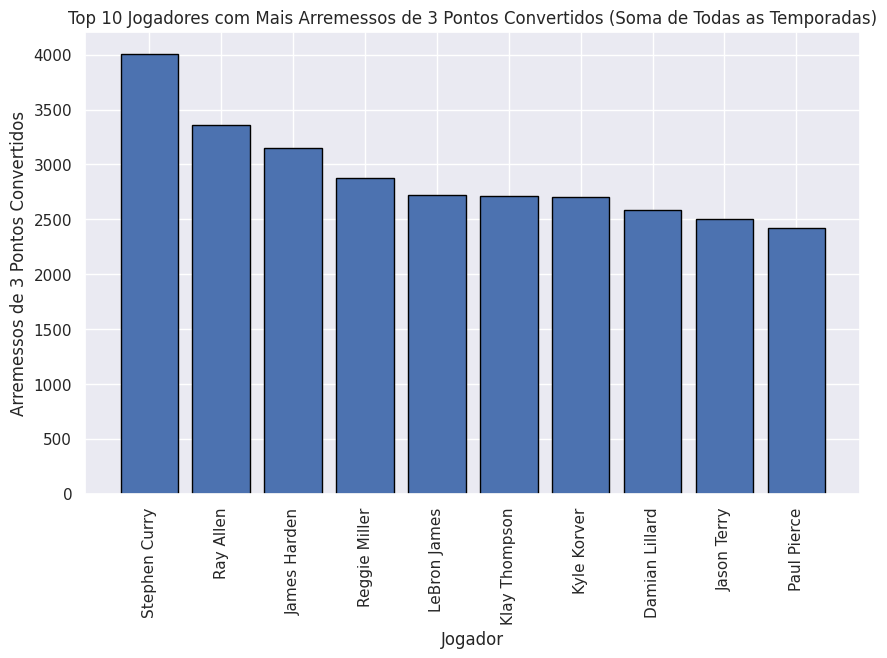
\includegraphics{imagens/19.png}

\hypertarget{o-que-define-um-time-bom}{%
\chapter{O que define um time bom?}\label{o-que-define-um-time-bom}}

\hypertarget{chernoff-faces}{%
\section{Chernoff Faces}\label{chernoff-faces}}

Últimos campeões e vices da NBA:

2013 - San Antonio Spurs \textbar{} Miami Heat

2014 - Golden State Warriors \textbar{} Cleveland Cavaliers

2015 - Cleveland Cavaliers \textbar{} Golden State Warriors

2016 - Golden State Warriors \textbar{} Cleveland Cavaliers

2017 - Golden State Warriors \textbar{} Cleveland Cavaliers

2018 - Toronto Raptors \textbar{} Golden State Warriors

2019 - Los Angeles Lakers \textbar{} Miami Heat

2020 - Milwaukee Bucks \textbar{} Phoenix Suns

2021 - Golden State Warriors \textbar{} Boston Celtics

2022 - Denver Nuggets \textbar{} Miami Heat

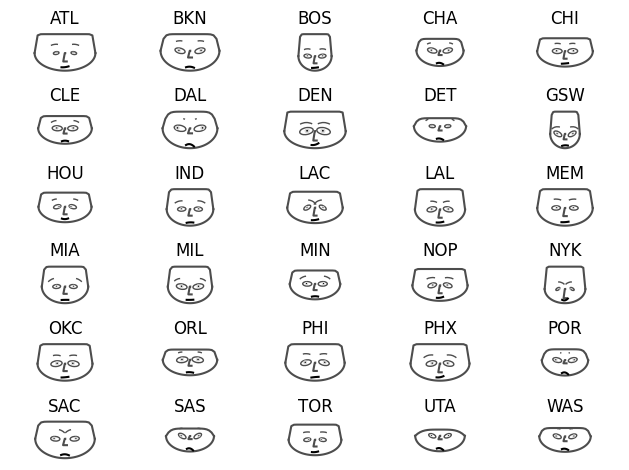
\includegraphics{imagens/20.png} 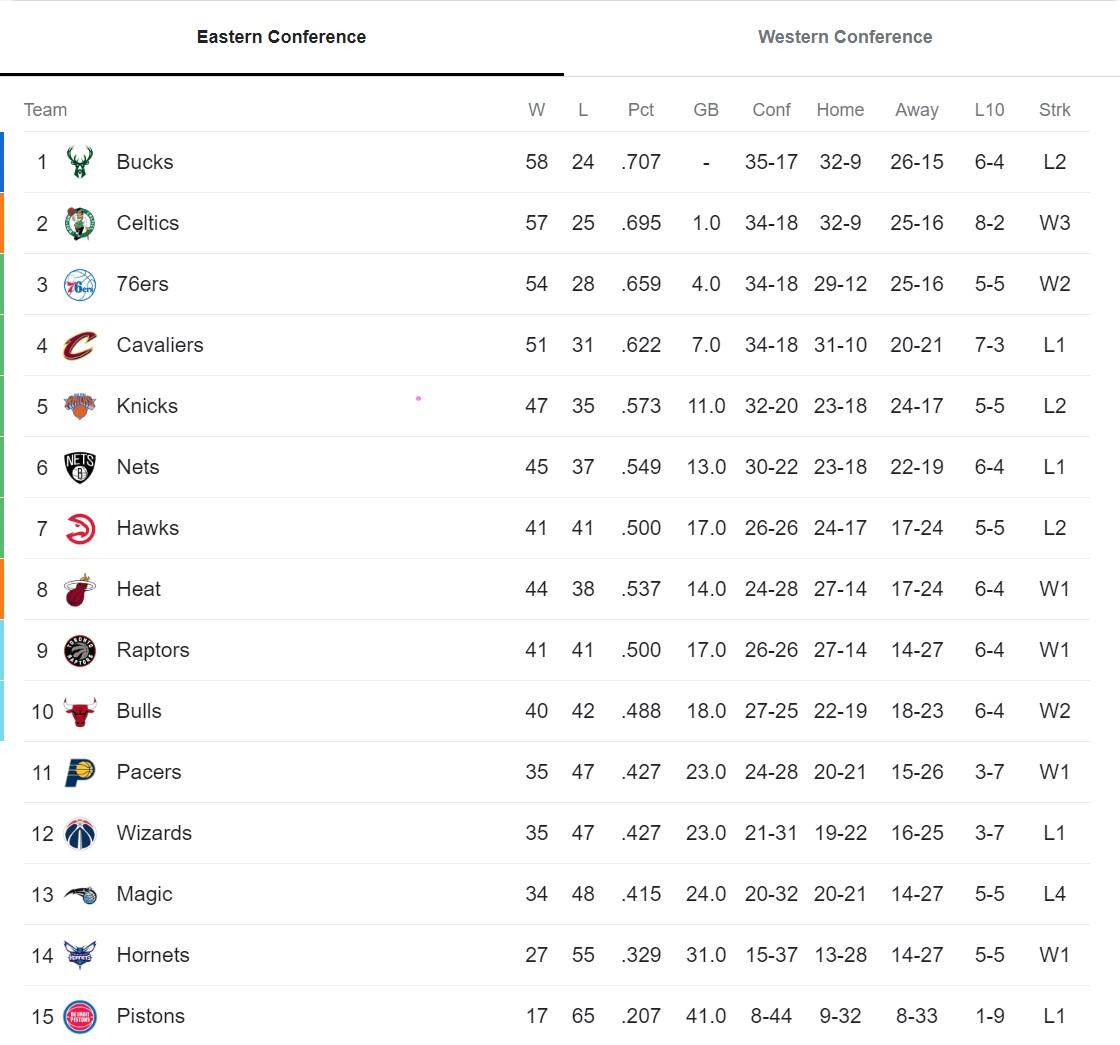
\includegraphics{imagens/21.jpeg} 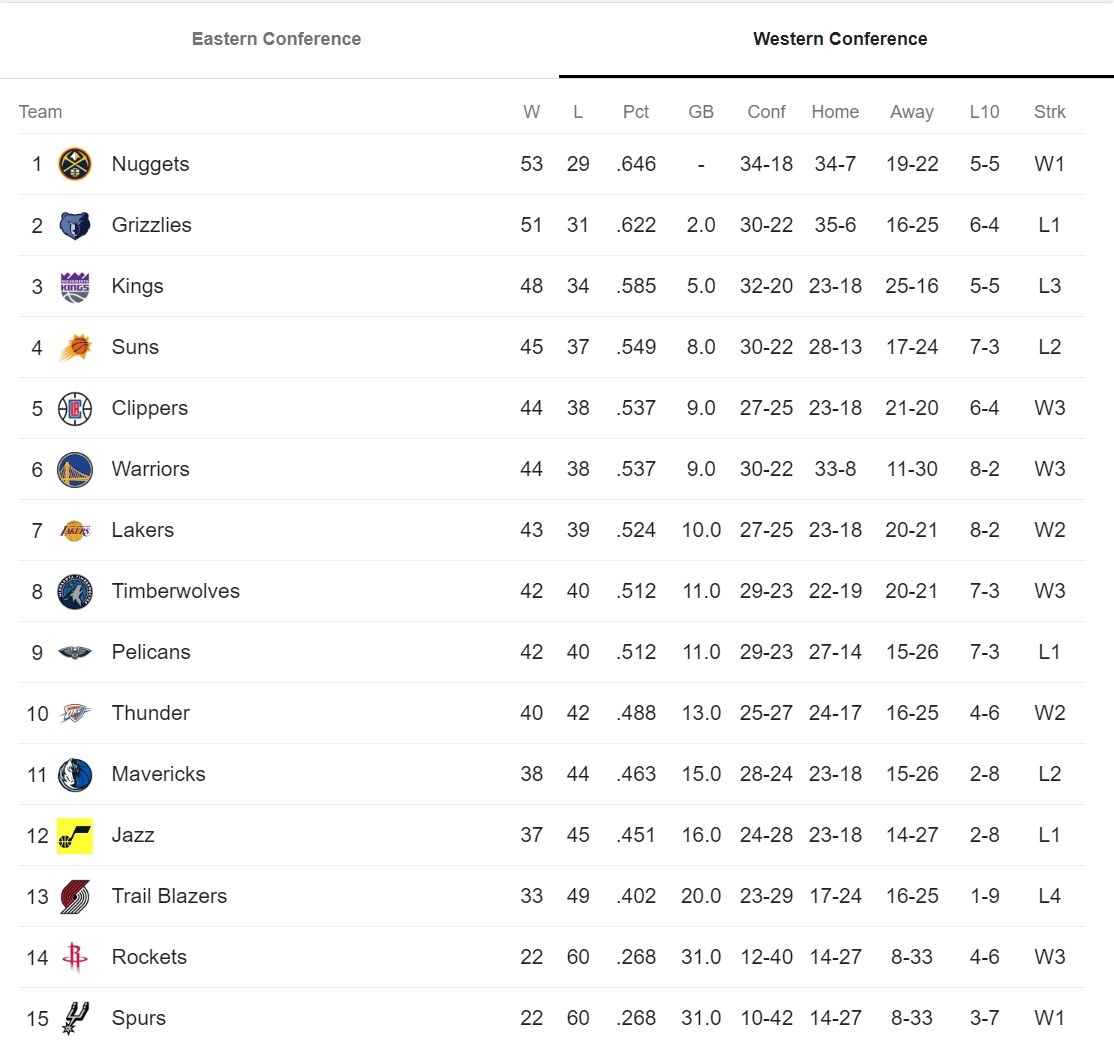
\includegraphics{imagens/22.jpeg} 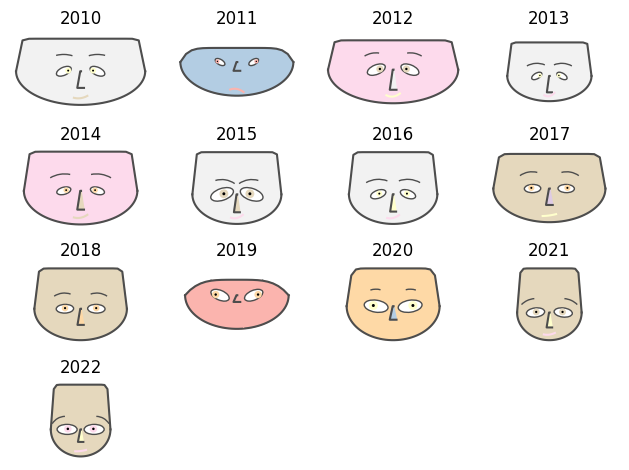
\includegraphics{imagens/23.png} Últimas posições na temporada regular do Golden State Warriors:

2010 - 3º

2011 - 4º

2012 - 2º

2013 - 2º

2014 - 1º

2015 - 1º

2016 - 1º

2017 - 1º

2018 - 1º

2019 - 5º

2020 - 4º

2021 - 2º

2022 - 4º

Concluindo, é possível observar tendencias de padrão e comportamento semelhantes em anos ou times que são parecidos, porém devido a natureza do gráfico e a falta de informação, principalmente para o ``usuário'' final, sobre os componentes representados por cada item (tamanho dos olhos, posição, inclinação da sobrancelha, etc.), não é possível fazer análises mais profundas.

Vemos como um gráfico de apoio para facilitar algumas visualizações ou fomentar questionamentos, por exemplo: os gráficos de 2015 e 2017 são significativamente diferentes, apesar do time ter sido campeão em ambas as temporadas. O desempenho nesses anos foi muito diferente? Ou então, os Pacers (IND) e os Wizards (WAS) tiveram o mesmo aproveitamento na temporada (0.427), porém seus gráficos são distintos. O que será que aconteceu? Sabemos que o resultado final de um jogo é apenas vitória ou derrota, porém a margem de pontos pode ser de 1 ou de 20, bem como a quantidade de arremesos, roubadas de bola, entre outros. Um time pode ter tido um desempenho comparável a times pior classificados e ter tido ``sorte'' de ganhar a quantidade suficiente de jogos, mesmo que por uma margem pequena e perder por muito, enquanto outro sempre tinha jogos parelhos, porém perdeu em mais ocasiões.

  \bibliography{book.bib,packages.bib}

\end{document}
